\section{Materials and Methods}
\label{sec:method}

\paragraph{TPMS lattice design.}
Three TPMS topologies were selected for this study based on their distinct geometric properties and relevance to heat transfer applications: Gyroid (G), Primitive (Schwarz-P), and IWP. Each topology was defined by its implicit level-set function. For the Gyroid surface, the level-set function is:
\begin{equation}
  f_G(\mathbf{x}) = \sin(x)\cos(y) + \sin(y)\cos(z) + \sin(z)\cos(x) = 0,
  \label{eq:gyroid}
\end{equation}
where $\mathbf{x} = (x, y, z)$ denotes the spatial coordinates normalized by the unit cell size. The Primitive and IWP surfaces are defined analogously with their respective level-set functions~\cite{tang2023analysis,himmelmann2026amorphous}. Fig.~\ref{fig:tpms} shows the three TPMS unit cell geometries. All lattices were designed with a unit cell size of 10~mm and a relative density of approximately 25\%, selected to balance structural integrity with PCM volume fraction.

\begin{figure}[htbp]
\centering
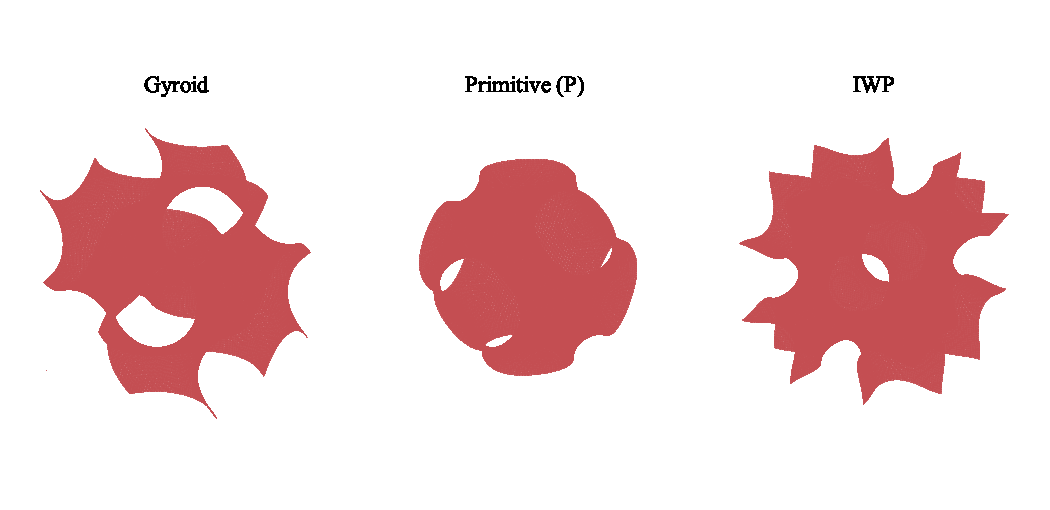
\includegraphics[width=\linewidth]{figures/fig_04_tpms_setup.pdf}
\caption{TPMS unit cell geometries investigated in this study: Gyroid, Primitive (Schwarz-P), and IWP surfaces rendered from their implicit level-set functions.}
\label{fig:tpms}
\end{figure}

\paragraph{Phase change material.}
A paraffin-based PCM with a nominal phase change temperature of 42\textdegree C was selected for this study. The PCM properties are: latent heat of fusion $L = 180$~kJ/kg, solid-state thermal conductivity $k_s = 0.25$~W/(m$\cdot$K), liquid-state thermal conductivity $k_l = 0.15$~W/(m$\cdot$K), density $\rho_s = 880$~kg/m$^3$, $\rho_l = 770$~kg/m$^3$, and specific heat $c_p = 2.1$~kJ/(kg$\cdot$K). These values are consistent with typical paraffin-based PCM properties reported in the literature~\cite{elarem2020thermal,abhat1983low,veerakumar2016phase}. The PCM was infiltrated into the TPMS lattice under vacuum to ensure complete filling of the interstitial voids.

\paragraph{Lattice fabrication.}
The TPMS lattice structures were fabricated from AlSiMg (AlSi10Mg) alloy using laser powder bed fusion (L-PBF) additive manufacturing. The L-PBF process parameters were optimized to achieve $>$99\% relative density: laser power 300~W, scan speed 1200~mm/s, layer thickness 30~$\mu$m, and hatch spacing 0.15~mm. The as-built lattice thermal conductivity was measured to be approximately 150~W/(m$\cdot$K), consistent with the expected value for AlSi10Mg~\cite{catchpole2019thermal,ghasemi2022unraveling}. The AlSiMg alloy was chosen for its excellent castability, high thermal conductivity, and proven suitability for L-PBF processing~\cite{rosenthal2015structure,mazur2017mechanical,nirsh2025mechanical}.

\paragraph{Sensor arrangement.}
Nine T-type thermocouples (T1--T9) were embedded within the TPMS/PCM composite at three distinct spatial groups to characterize the temperature field distribution (Fig.~\ref{fig:setup}):
\begin{itemize}[nosep]
  \item Group A: $T_1$ --- positioned nearest to the heating element
  \item Group B: $T_2$--$T_5$ --- positioned at intermediate radial distance
  \item Group C: $T_6$--$T_9$ --- positioned at the outermost radial distance
\end{itemize}
This arrangement enables characterization of the radial thermal gradient from the heat source through the TPMS/PCM composite. A schematic of the sensor layout is shown in Fig.~\ref{fig:setup}.

\begin{figure}[htbp]
\centering
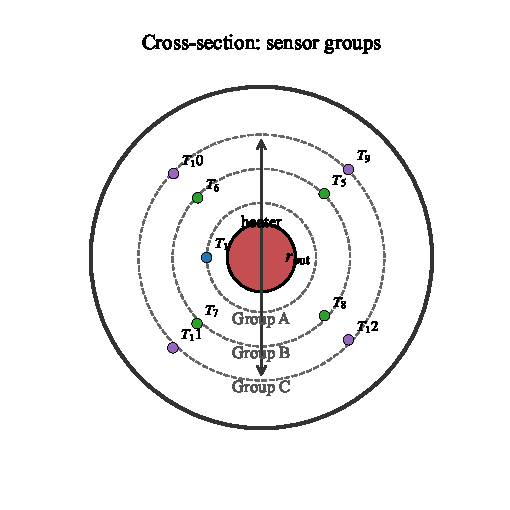
\includegraphics[width=0.5\linewidth]{figures/fig_05_setup.pdf}
\caption{Cross-section schematic of the experimental specimen showing the central cartridge heater and the three thermocouple groups (A: $T_1$; B: $T_2$--$T_5$; C: $T_6$--$T_9$) at increasing radial distances.}
\label{fig:setup}
\end{figure}

\paragraph{Data processing.}
Temperature data were acquired at 1~Hz sampling rate. To address sensor-to-sensor variability, a two-stage data processing pipeline was applied~\cite{piacquadio2022experimental}: (1)~spatial outlier removal---within each group, the sensor exhibiting the largest time-averaged deviation from the group mean was identified and excluded, with the remaining sensors averaged; (2)~temporal smoothing---an exponential moving average (EMA) filter with $\alpha = 0.4$ (time constant $\approx$2.5~s) was applied to suppress high-frequency noise while preserving the thermal transient characteristics:
\begin{equation}
  \bar{T}_t = \alpha \, T_t + (1 - \alpha)\,\bar{T}_{t-1}.
  \label{eq:ema}
\end{equation}
where $T_t$ is the raw group mean at time step $t$ and $\bar{T}_t$ is the smoothed value.
